\section{System Identification}\label{sec:system_id}
Section~\ref{sec:modelling} left three constants unmeasured: the plant gain $A$, the time constant
$T$ and the sensor constant $k$. This section reports the tests that fixed them.

\subsection{Method}
The plant is first order at velocity level and second order at position level, so the tests are
built around Equation~\eqref{eqn:openloop_vel} rather than Equation~\eqref{eqn:openloop_pos}.

\paragraph{Hover voltage.} The input was raised until the kitticopter held height with its
vertical speed below $0.02\ \mathrm{m\,s^{-1}}$, where thrust exactly cancels gravity. This is the
zero point of the controller and the baseline of every step test; stepping from $0\ \mathrm{V}$
would start the kitticopter in free fall and the trace would not be a step response of the linear
model. Measured twice, at $2.495$ and $2.515\ \mathrm{V}$.

\paragraph{Input circuit.} Steps were commanded from a breadboard divider off the
$15\ \mathrm{V}$ rail: $56\ \mathrm{k\Omega}$ to a trimmer, $12\ \mathrm{k\Omega}$ to ground,
wiper to ADC input 1. Its range is bounded to keep the command inside the $0$ to $5\ \mathrm{V}$
window the plant accepts, since above $5\ \mathrm{V}$ the excess is ignored and the commanded step
would be larger than the one the plant actually saw.

\paragraph{Velocity.} The rig logs time, input voltage, output voltage and position, but no
velocity, so velocity comes from differentiating the logged position with a centred difference,
\begin{equation}\label{eqn:central_difference}
    v_n = \frac{h_{n+1} - h_{n-1}}{t_{n+1} - t_{n-1}} .
\end{equation}
at a $100\ \mathrm{ms}$ sample interval.

\paragraph{Extraction.} From each settled response the gain is the ratio of final velocity to step
size, and the time constant the time to reach $63.2$ percent of that final value:
\begin{equation}\label{eqn:AT_extraction}
    A = \frac{v_\infty}{V_2 - V_h},
    \qquad
    v(T) = 0.632\,v_\infty .
\end{equation}
A second estimate of $T$ comes from fitting a straight line to $\ln(v_\infty - v)$ against time,
whose slope is $-1/T$. The two estimates are reported together as a check on each other.

\paragraph{Sign of the difference.} Equation~\eqref{eqn:central_difference} is signed, not a
magnitude. A climb gives a positive velocity and a fall a negative one, and the decay tests depend
on that: absolute values would fold the decay back on itself and make the fitted time constant
meaningless.

\paragraph{Choice of interval.} The differencing interval is a judgement rather than a constant,
and it was chosen differently in different parts of each run. The logged position is quantised, so
over one $100\ \mathrm{ms}$ sample that quantisation is a significant fraction of the few metres
travelled and the velocity is noisy; widening the interval averages it away, because the same
quantisation is negligible against a change of hundreds of metres. But a wide interval also
averages across curvature, and during the transient the curvature is the signal being measured.

The resolution is to match the interval to the region. On the settled plateau the curve is
straight, so tens of seconds are used, which is what Equation~\eqref{eqn:dhdt_worked} does.
Through the transient a centred difference over neighbouring samples is used instead and the extra
noise accepted. One interval everywhere would either corrupt the plateau with noise or flatten
the transient, and both errors land directly on $A$ and $T$.

\paragraph{Gain from a regression, not a single run.} Each run on its own gives a gain by
Equation~\eqref{eqn:AT_extraction}, but that ratio assumes the hover voltage is exactly right: an
error in $V_h$ shifts every step size by the same amount and biases the gain. Fitting the settled
velocities of all the runs against input voltage instead removes the assumption and returns the
hover voltage as a result, as Equation~\eqref{eqn:gain_regression} does.

\paragraph{Time constant from the position curve, not the velocity curve.} Reading the $63.2$
percent level requires a velocity signal, which requires differentiating the log and therefore
amplifying its quantisation. Fitting the analytic position response of
Equation~\eqref{eqn:height_fit} instead uses the raw logged column with no differentiation at all,
and uses every sample rather than the single crossing point. It is the better conditioned of the
two routes, so it is the one reported, with the $63.2$ percent reading kept as the check.

\paragraph{Decay tests as validation, not as measurement.} In a step test $A$ and $T$ are pulled
from the same curve, so an error in one can hide inside the other and the fit still looks good.
Stepping the input back down to hover breaks that coupling: the velocity decays toward zero, there
is no final value for the gain to influence, and what remains depends on $T$ alone. That is why
the decay result is reported as a check on the model rather than averaged into it.

\subsection{Results}
Eight runs are used: seven step tests at four step sizes, with the two smallest and the largest repeated, plus the full-range test of Section~\ref{sec:system_id}.
Table~\ref{tab:stepruns} lists them. Figure~\ref{fig:step_response} shows the velocity responses
aligned at the step, and the linearity check described below.


\begin{figure}[htbp]
    \centering
    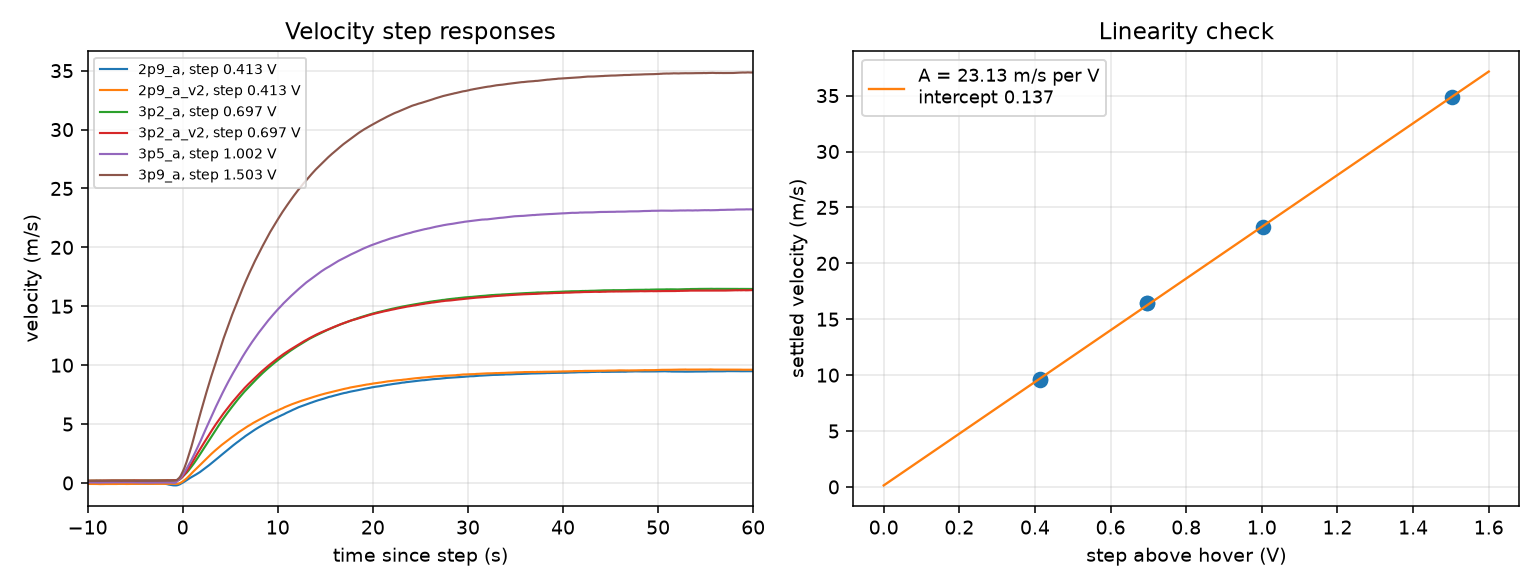
\includegraphics[width=0.62\textwidth]{figures/step_response.png}
    \caption{Left: velocity against time for the seven step runs, aligned at the instant of the step.
    Each settles to a constant, as a first-order response should, with no overshoot. Right:
    settled velocity against raw input voltage. The straight line has slope $23.196$ and crosses
    zero velocity at $2.5016\ \mathrm{V}$, recovering the hover voltage without it having been
    assumed.}
    \label{fig:step_response}
\end{figure}

\paragraph{Gain and hover voltage from one fit.} The individual ratios in
Table~\ref{tab:stepruns} each divide by $V_{in} - V_h$, so each one inherits whatever error is in
the hover voltage. Regressing the settled velocity against the \emph{raw} input voltage removes
that dependence, because

\begin{equation}
    v_\infty = A\left(V_{in} - V_h\right) = A\,V_{in} - A V_h ,
\end{equation}
so the slope is the gain and the horizontal intercept is the hover voltage. Neither is assumed;
both are fitted. Over the eight runs,
\begin{align}\label{eqn:gain_regression}\begin{split}
    A = \frac{n\sum V_{in}v_\infty - \sum V_{in} \sum v_\infty}
             {n \sum V_{in}^2 - \left(\sum V_{in}\right)^2}
      = \frac{8(797.959) - (28.6512)(200.379)}{8(106.0741) - (28.6512)^2} \\
      = \frac{642.572}{27.7015}
      = 23.196\ \mathrm{m\,s^{-1}V^{-1}} ,
\end{split}\end{align}
\begin{equation}
    V_h = -\frac{c}{A} = \frac{58.0278}{23.196} = 2.5016\ \mathrm{V} .
\end{equation}
The residuals are $+0.020$, $-0.023$, $-0.029$, $+0.015$, $-0.008$, $+0.040$, $+0.005$ and
$-0.019\ \mathrm{m\,s^{-1}}$, an rms of $0.022$ against velocities reaching $57.9$. Two things
follow. The plant is linear over the whole $0$ to $5\ \mathrm{V}$ range, since one straight line
fits a sixfold spread of step sizes to within the logging resolution. And the fitted hover voltage
lands on $2.50\ \mathrm{V}$, the midpoint of the input range, which the brief states is where
thrust cancels gravity by design. That value was never put into the fit, so its appearance in the
answer is an independent check on the whole measurement rather than a restatement of an
assumption.

\paragraph{Sensor constant.} The rig logs position in both volts and metres, so $k$ follows from
the ratio of the two columns. Only samples below $9.9\ \mathrm{V}$ were used, because the sensor
output saturates at $10\ \mathrm{V}$ near a height of $10.5\ \mathrm{m}$ while the metre column
continues to read truthfully. Every run gives the same value,
\begin{equation}
    k = 0.9500\ \mathrm{V\,m^{-1}} .
\end{equation}

\subsection{Full-range test}
A final test used the largest step the rig allows, from hover straight to the $5\ \mathrm{V}$
ceiling. Pushing the potentiometer hard against its end stop made the input move from $2.967$ to
$5.000\ \mathrm{V}$ within a single $100\ \mathrm{ms}$ sample, so unlike the earlier runs there is
no ramp to distort the early part of the response. It was held for $185\ \mathrm{s}$, by which
point the velocity was flat to three decimals at $57.935\ \mathrm{m\,s^{-1}}$ and the simulator
reported zero lift, the signature of terminal velocity where thrust balances gravity and drag
together.

\paragraph{Reading the velocity.} Applying the interval rule above to the settled region, two
points $29.9\ \mathrm{s}$ apart late in the run give
\begin{equation}\label{eqn:dhdt_worked}
    v = \frac{3341.697 - 2298.690}{2443.7 - 2413.8} = \frac{1043.007}{29.9}
      = 34.88\ \mathrm{m\,s^{-1}} ,
\end{equation}
stable to three figures, against the same quantity computed over one sample, which scatters by
several $\mathrm{m\,s^{-1}}$.

\paragraph{Gain.} With the fitted hover voltage of $2.5016\ \mathrm{V}$,
\begin{equation}
    A = \frac{57.935}{5.0000 - 2.5016} = 23.197 ,
\end{equation}
which agrees with the regression of Equation~\eqref{eqn:gain_regression} to $0.001$. Taking
hover at its design value of exactly $2.5\ \mathrm{V}$ instead gives $23.174$, a difference of
$0.1$ percent, so the choice no longer matters once the hover voltage is fitted rather than
trimmed by eye.

\paragraph{Time constant.} Two routes were used. Reading the $63.2$ percent level off the velocity
curve gives $0.632 \times 57.935 = 36.615\ \mathrm{m\,s^{-1}}$, crossed at $t = 9.542\ \mathrm{s}$
after the step. Alternatively the analytic step response of the position,
\begin{equation}\label{eqn:height_fit}
    h(t) = v_\infty \left( t - T \left( 1 - e^{-t/T} \right) \right) ,
\end{equation}
was fitted by least squares to all $1800$ logged samples, which avoids differentiating the signal
at all and therefore avoids amplifying its noise. That gives $T = 9.537\ \mathrm{s}$ and
$v_\infty = 57.931\ \mathrm{m\,s^{-1}}$, with an rms residual of $0.403\ \mathrm{m}$ against
$9869\ \mathrm{m}$ of travel. The two routes agree to $0.1$ percent.

The fit also shows how sharply $T$ is determined. Holding the fit at $T = 9.50$ raises the
residual to $0.92\ \mathrm{m}$ and at $T = 9.70$ to $3.75\ \mathrm{m}$, so a $2$ percent error in
$T$ is already an order of magnitude worse than the optimum. This matters in
Section~\ref{sec:design}, where the gain window is narrow enough that the plant parameters have to
be trusted to better than the $10$ percent the specification allows for.

\subsection{Model validation}
Two independent checks were made on the identified model.

\paragraph{Decay test.} In a step test the gain and the time constant come from the same curve, so
an error in one can be absorbed by the other. Returning the input to hover breaks that coupling,
because the velocity then decays with no final value for the gain to influence. Both logs recorded
for this turned out to hold the whole bench session rather than one event, with $14$ and $28$
separate input changes, so one was discarded and a single clean $164\ \mathrm{s}$ segment was
fitted from the other, with the final velocity free rather than assumed to be zero. Details are in
Appendix~\ref{sec:appendix}. It gives $T = 9.163\ \mathrm{s}$, rms residual
$0.113\ \mathrm{m\,s^{-1}}$ over $1640$ samples, which is $3.9$ percent below the step-test value
and is carried into the uncertainty below.

The same fit returns a residual velocity of $0.157\ \mathrm{m\,s^{-1}}$, while the input over that
segment averaged $2.5080\ \mathrm{V}$ and the identified constants predict
$23.196 \times (2.5080 - 2.5016) = 0.149\ \mathrm{m\,s^{-1}}$. The two agree to
$0.008\ \mathrm{m\,s^{-1}}$. This is the strongest check in the identification: a small number
predicted from two constants measured elsewhere, in a part of the data that played no part in
measuring them.

\paragraph{Independent reimplementation.} The entire analysis was carried out twice, once in
Python and once in MATLAB, written separately against the same raw logs. The two agree on $A$,
$T$ and $k$ to three decimal places.

\subsection{Identified model}
\begin{equation}\label{eqn:identified}
    A = 23.196\ \mathrm{m\,s^{-1}V^{-1}}, \qquad
    T = 9.537\ \mathrm{s}, \qquad
    k = 0.9500\ \mathrm{V\,m^{-1}} ,
\end{equation}
so the velocity plant of Equation~\eqref{eqn:openloop_vel} and the position plant of
Equation~\eqref{eqn:openloop_pos} become
\begin{equation}
    \frac{V(s)}{F_t(s)} = \frac{23.196}{9.537s + 1},
    \qquad
    G(s) = \frac{23.196}{s\left(9.537s + 1\right)} .
\end{equation}
The corresponding drag constant is $b = 1/T = 0.10485\ \mathrm{s^{-1}}$, and the thrust constant $a = A/T = 2.4322\ \mathrm{m\,V^{-1}s^{-2}}$.

The figures are carried to three decimals because the design window in
Section~\ref{sec:design} is narrow, but the honest uncertainty is wider than that. The gain is now
the better determined of the two: the regression residual is $0.022\ \mathrm{m\,s^{-1}}$ and the
four routes to $A$ span $23.19$ to $23.22$, so $A = 23.20 \pm 0.03$. The time constant is less settled. The height-curve fit gives $9.537\ \mathrm{s}$ and rejects
anything far from it, trebling its residual at $9.60$, while the independent decay fit gives
$9.163$. The two methods therefore disagree by $3.9$ percent, which is larger than either one's own
scatter, so the defensible statement is $T = 9.5 \pm 0.4$ rather than the tighter figure the
step-test fit alone would suggest. The sensor constant is known to four figures. These uncertainties are carried into the
corner analysis of Section~\ref{sec:design}, where the specification requires robustness to
$10$ percent in the drag constant anyway, which is far wider than either.
The model was also submitted to the parameter-check tool of Appendix~A2 of the brief, which
scores it against the values the simulator was generated from. That exercise and its outcome are
reported in Appendix~\ref{sec:appendix}, since it tests the measurement rather than forming part
of it.
